\section{Introduction}
\IEEEPARstart{I}{ndustrial} production systems expose measurements and control
points through interfaces that vary by process line, device, and communication
protocol. A task-level agent therefore needs more than a list of tools: it must
receive the active line, product, recipe, and run context, address the intended
control node, and operate within the limits configured for that process. A
command receipt also has a different meaning from a subsequent process
measurement. In the cast-film simulator used in this study, for example, line
speed is configured through a message-queuing protocol while film thickness is
acquired as a process value. In the evaluated scene, the MQTT endpoint carries
the line-speed setpoint and returns thickness samples; this configured pairing
does not by itself establish that a write caused a measured change. The
architecture must preserve the relation between those signals without treating
a successful write as proof of a desired process response.

Research on industrial agents addresses process supervision, control
generation, service selection, and human-guided automation
\cite{xia2025control,huang2026made,koehle2026llmdriven,biskupovic2025supervision,
liu2026agents4plc,wu2025instructmpc,lim2025llmenabled,zhao2026shopfloor,
hofmann2025nlc}. Other work connects agents with digital twins, manufacturing
skills, and shop-floor services
\cite{xia2025architecture,silva2025mcpmanufacturing,
koehle2025semanticrecipes,graul2026aas,schall2026safe,lin2026agentic}.
Industrial-informatics architectures have also formalized trust boundaries for
digital-twin control, functional blocks for industrial IoT networks, and
security services at the fog layer
\cite{gehrmann2020dtiacs,mahmood2023functional,sengupta2021securefog}.
Together, these studies provide methods for agent reasoning, asset grounding,
communication, and secure service execution. They motivate a complementary
deployment question: how should a system bind different production scenes and
agent runtimes to the same governed operation boundary?

This work addresses that integration boundary. It designs and implements a
configuration-driven architecture in which production context and
protocol-specific I/O are defined by scene configuration, while harness
adapters present agent engines through a common task-operation interface.
Task-mediated calls and direct operation calls converge on shared dispatch
checks, and each device write is evaluated against the live context and the
limits configured for its route. The contribution is a system architecture
and its implementation, rather than a new control law or an autonomous-agent
algorithm.

The paper makes two architectural contributions:
\begin{enumerate}
  \item A scene configuration binds line--product--recipe--run context to
  semantic data-acquisition and write-control nodes, protocol drivers,
  objectives, and engineering limits. The mappings remain explicit per scene
  behind a common operation interface.
  \item A task-to-device runtime separates harness turn execution from
  scene-specific I/O. Task calls and direct operation calls enter a shared
  dispatcher, which checks authority and current context before route-specific
  limits and any required approval are applied. Service-owned records keep
  command receipts distinct from later process observations.
\end{enumerate}

The evaluation tests selected links across this architecture in a deterministic
simulator execution. Its scope and evidence limits are stated with the results;
the run does not establish real-harness interchangeability or field operation.

Section~II positions the integration problem among industrial-agent and
industrial-informatics architectures. Section~III describes the system
architecture and execution contract, and Section~IV details context assembly,
write admission, approval revalidation, and record semantics. Section~V
reports distinct evidence blocks from the single simulator execution:
workflow coverage, protocol acquisition and guard checks, seeded objective
cases, and a separately scripted BOPET integration trace. Sections~VI and
VII discuss what these observations support and where the evidence ends.

Fig.~\ref{fig:control-path} summarizes how scene-bound context and I/O mappings
meet the shared dispatch boundary before a configured driver is invoked.

\begin{figure}[!b]
\centering
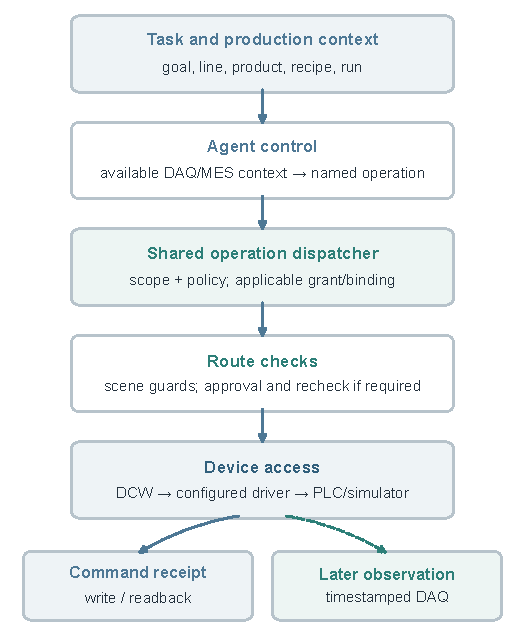
\includegraphics[width=\columnwidth]{resources/fig1-nature-A.pdf}
\caption{Task execution from process context to device observation. Data
acquisition (DAQ) and manufacturing execution system (MES) services provide
process context for a named operation. Shared
dispatch checks precede route-specific limits and any required approval and
context revalidation. Configured drivers access the device; the command
receipt and later process measurement remain separate records.}
\label{fig:control-path}
\end{figure}
